\section{Introduction}
\label{sec:intro}

Alongside exploration tasks, the importance of developing teleoperated mobile systems has been recognized for a long time. Historically, humans have conducted exploration missions themselves, which remains effective for many low-risk and specific tasks. 
However, for higher-risk and more hazardous missions—such as volcanic surveys or planetary exploration—researchers rely on specialized vehicles known as \textit{rovers}.
For example, \href{https://www.nasa.gov/}{NASA} launched the \href{https://science.nasa.gov/mission/mer-opportunity/}{Opportunity} in 2003 and the \href{https://science.nasa.gov/mission/msl-curiosity/}{Curiosity} in 2012, two of the longest-operating missions on Mars, aimed at determining whether the planet could have supported life.

\par
Although each rover was designed for different specific missions and utilized distinct technologies, 
they share several common structural features. Both systems were designed to be controlled and monitored 
from NASA headquarters on Earth. Additionally, they were engineered for high reliability and strong terrain 
adaptability—key factors that serve as motivation for the development of our own rover platform.


\begin{figure}[h]
    \centering
    \begin{subfigure}{0.45\textwidth}
        \centering
        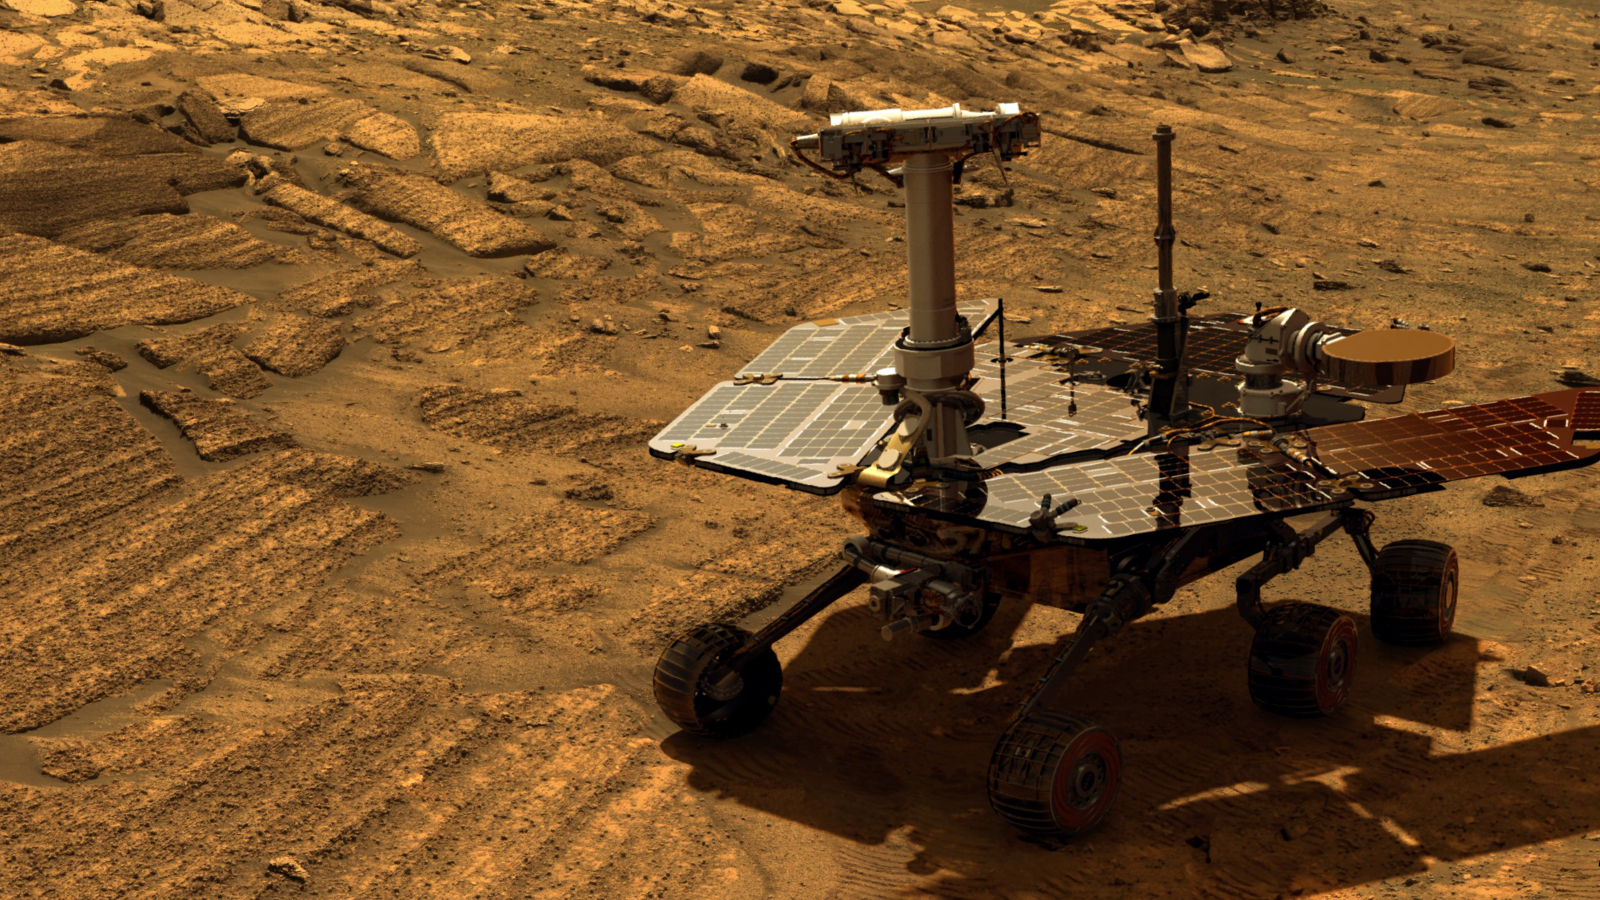
\includegraphics[width=\linewidth]{images/rover_reference /opportunity.jpg}
        \caption{Opportunity Rover}
        \label{fig:opportunity}
    \end{subfigure}
    \hfill
    \begin{subfigure}{0.45\textwidth}
        \centering
        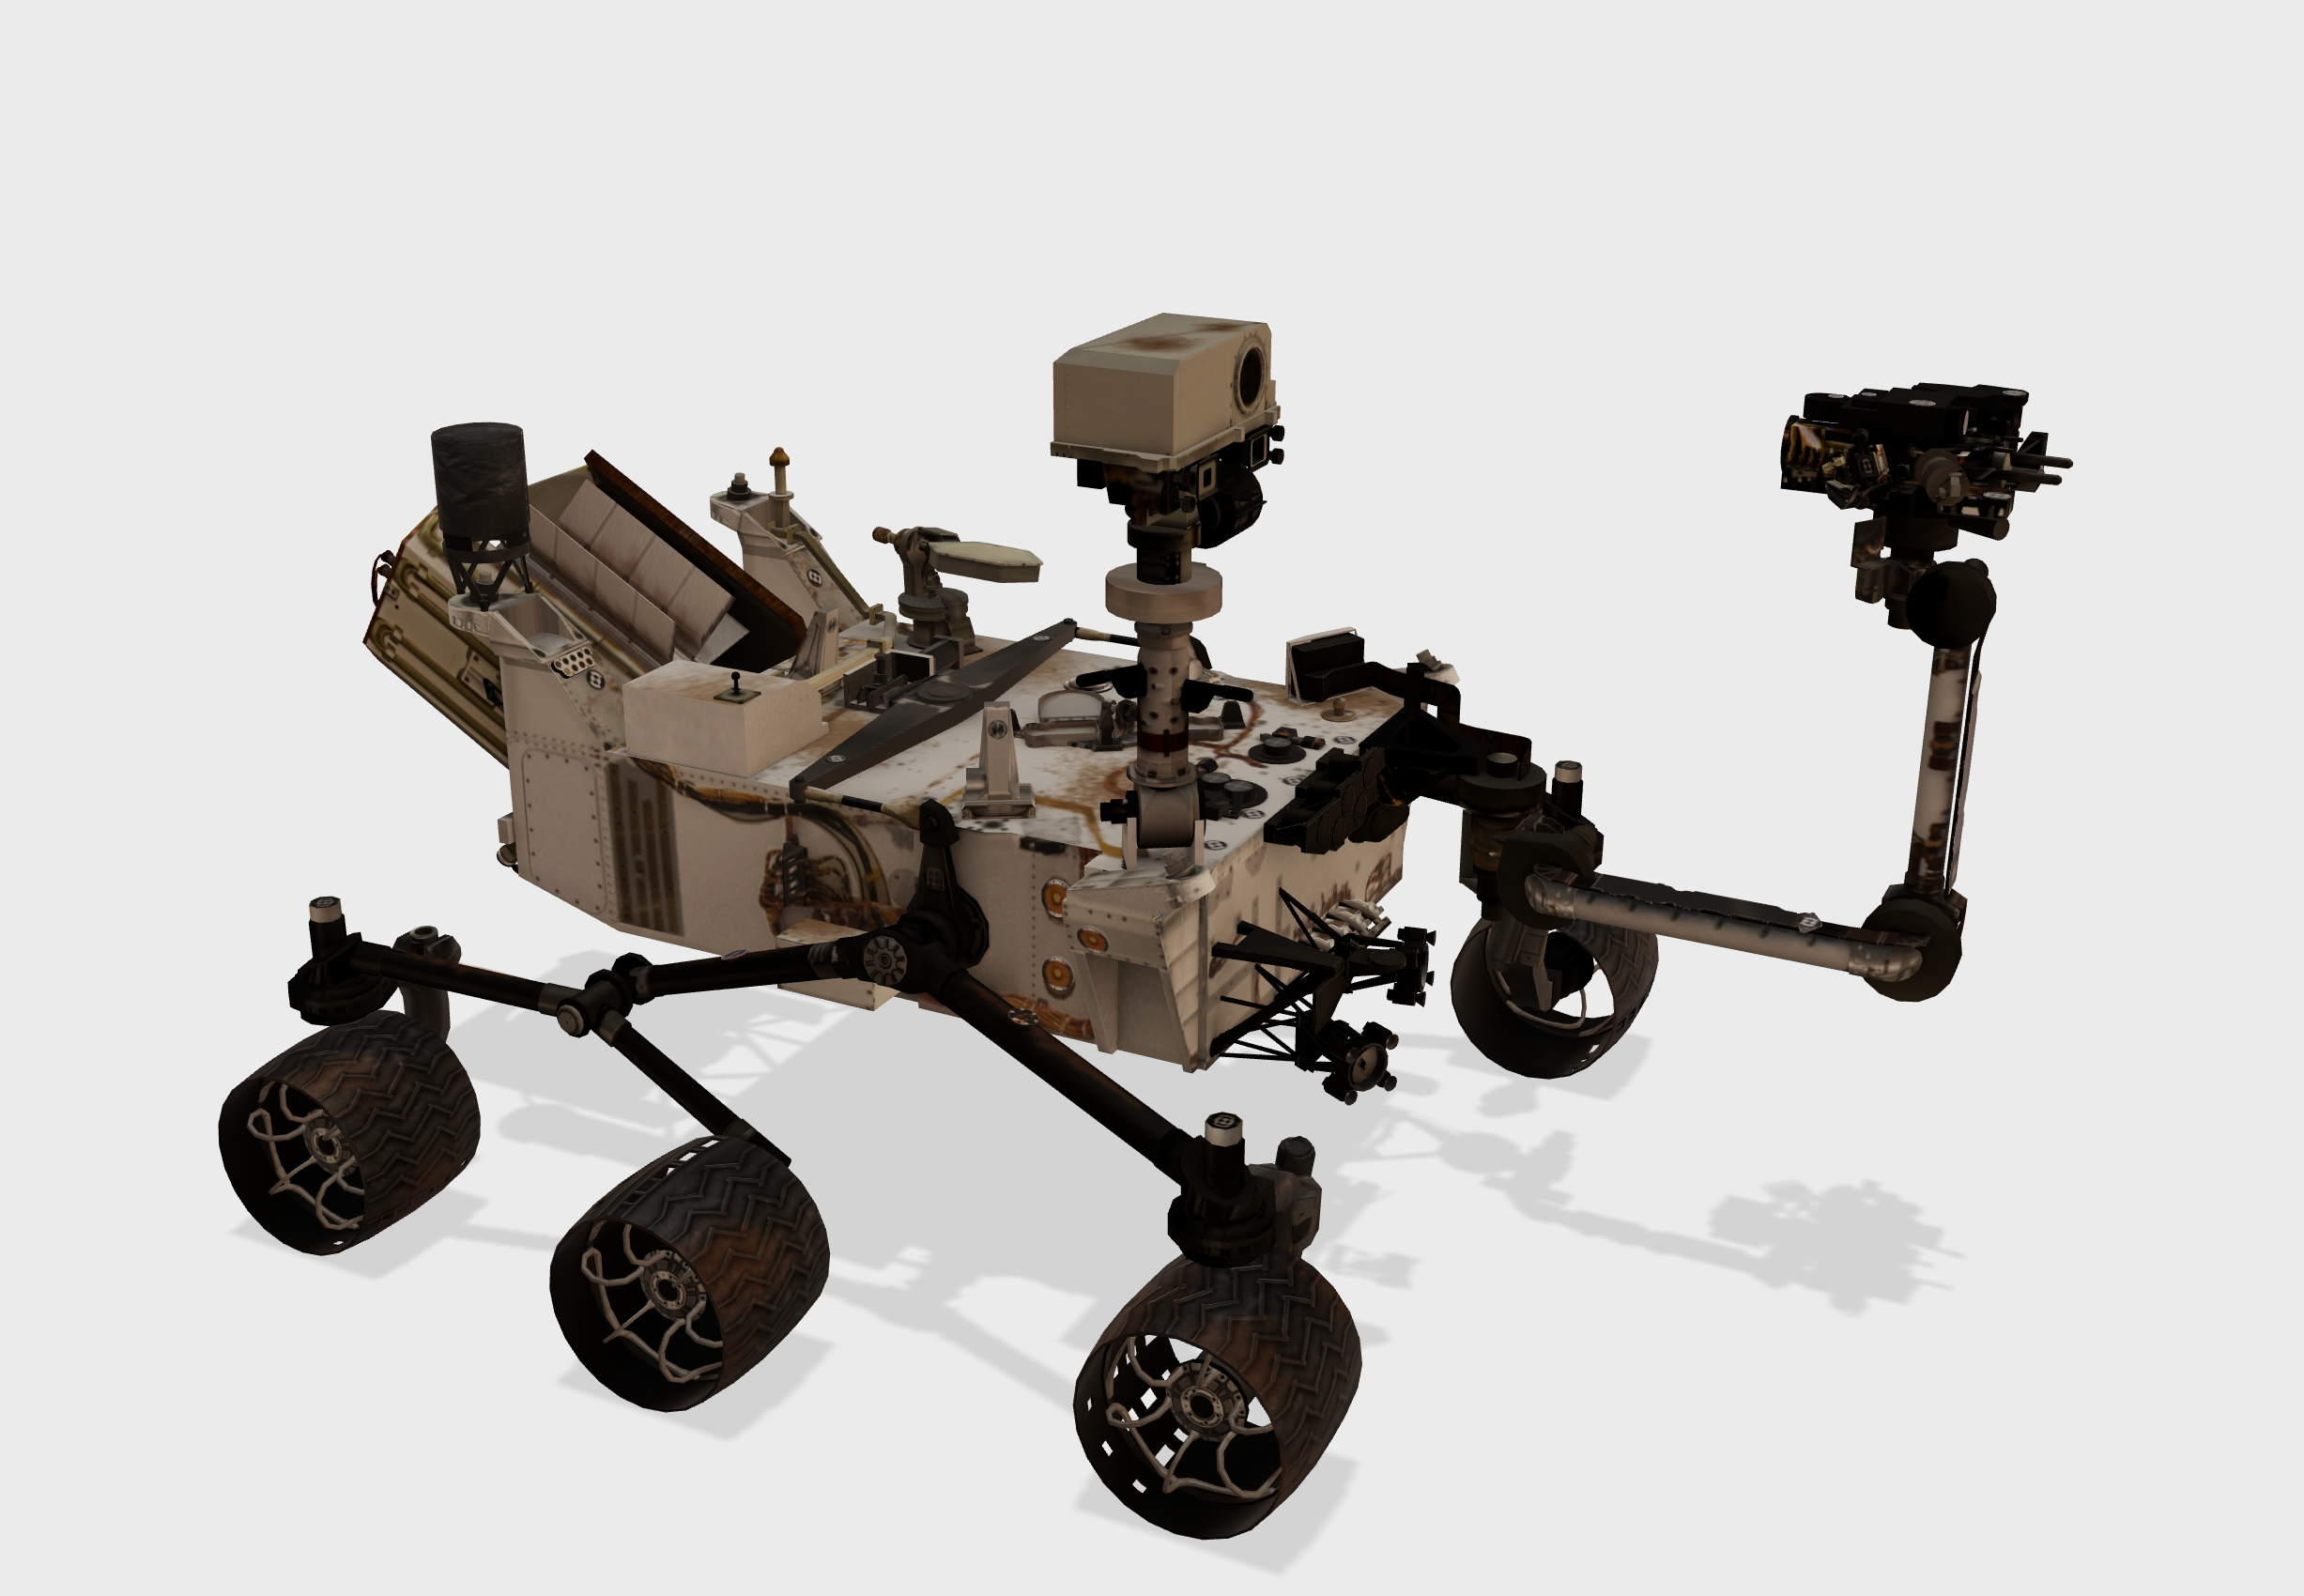
\includegraphics[width=\linewidth]{images/rover_reference /curiosity.png}
        \caption{Curiosity Rover}
        \label{fig:curiosity}
    \end{subfigure}
    
    \caption{Curiosity and Opportunity Rovers hold record for two longest operating time, 
    14 years (~5100 Sols) for Opportunity and 13.7 years (4863 Sols) for Curiosity.}
    \label{fig:rovers}
\end{figure}


This section introduces our rover platform, MAVEN-01, which represents the first iteration of our design. 
We are currently continuing its development to improve performance, durability, and reliability. 
Through multiple prototypes and design iterations—including unsuccessful attempts—MAVEN-01 has evolved with a clear objective: 
to provide a low-cost rover platform for research and experimental purposes using 3D printing technology.
The rover is designed to support customization for specific tasks, featuring multiple mounting holes 
on the top surface to accommodate additional components and modules.





